\subsection{Agenda}
%%%%%%%%%%%%%%%%%%%%%%%%%%%%%%%%%%%%%%%%%%%%%%%%%%%%%%%%%%%%%%%%%%%%%%%%%%%%%%%%%%%%%%%%%%%%%%%%%%% 
\begin{frame}
	\frametitle{Quantum crypanalysis}
		\framesubtitle{Agenda}
	\vspace{-1cm}
	\hspace{-1.5cm}{	
	\begin{description}
		\item[1.]{Bra-ket notation}
		\item[2.]{Quantum gates}
		\item[3.]{Grover's database search}
		\item[4.]{Shore's factorization algorithm}
    	\begin{enumerate}
           \item[•]{ Fast modular exponentiation}\\
           \item[•]{ Quantum Fourier transform}\\
    	\end{enumerate}
		\item[5.]{Implementation of quantum computer}
		\item[6.]{Summary}
	\end{description}
	}
\end{frame}

%%%%%%%%%%%%%%%%%%%%%%%%%%%%%%%%%%%%%%%%%%%%%%%%%%%%%%%%%%%%%%%%%%%%%%%%%%%%%%%%%%%%%%%%%%%%%%%%%%%	

\subsection{Notation and properties}
%%%%%%%%%%%%%%%%%%%%%%%%%%%%%%%%%%%%%%%%%%%%%%%%%%%%%%%%%%%%%%%%%%%%%%%%%%%%%%%%%%%%%%%%%%%%%%%%%%% 
\begin{frame}
	\frametitle{Bra-ket notation}
		\framesubtitle{Definition}
		\vspace{-1cm}
	{\normalsize
	\hspace{0.5cm}{Bra–ket notation, also known as Dirac notation: $\braket{x|y}$ is a standard notation for describing quantum states. It can also be used to denote abstract vectors, linear functionals and scalar product in mathematics.}\\
	\vspace{0.4cm}
	\hspace{0.0cm}{The left part: $\bra{x}$, called the bra, is a row vector.}\\
	\hspace{0.0cm}{The right part: $\ket{y}$, called the ket, is a column vector.}\\
	\hspace{0.5cm}{}\\

	}
\end{frame}
%%%%%%%%%%%%%%%%%%%%%%%%%%%%%%%%%%%%%%%%%%%%%%%%%%%%%%%%%%%%%%%%%%%%%%%%%%%%%%%%%%%%%%%%%%%%%%%%%%%

%%%%%%%%%%%%%%%%%%%%%%%%%%%%%%%%%%%%%%%%%%%%%%%%%%%%%%%%%%%%%%%%%%%%%%%%%%%%%%%%%%%%%%%%%%%%%%%%%%% 
\begin{frame}
	\frametitle{Qbit}
		\framesubtitle{Definition}
		\vspace{-1cm}
	{\normalsize
	A pure qubit state is a linear superposition of the basis states. This means that the qubit can be represented as a linear\\ combination of $|0\rangle$ and $|1\rangle $:\\ 
    $|\psi \rangle =\alpha |0\rangle +\beta |1\rangle$\\
  
    When we measure this qubit in the standard basis, the probability of outcome $|0\rangle$  is $|\alpha |^{2}$ and the probability of outcome $|1\rangle$  is $|\beta |^{2}$. Because the absolute squares of the amplitudes equate to probabilities, it follows that
     $\alpha$ and $\beta$ must be constrained by the equation
$$|\alpha |^{2}+|\beta |^{2}=1$$\\
	}
\end{frame}
%%%%%%%%%%%%%%%%%%%%%%%%%%%%%%%%%%%%%%%%%%%%%%%%%%%%%%%%%%%%%%%%%%%%%%%%%%%%%%%%%%%%%%%%%%%%%%%%%%%

%%%%%%%%%%%%%%%%%%%%%%%%%%%%%%%%%%%%%%%%%%%%%%%%%%%%%%%%%%%%%%%%%%%%%%%%%%%%%%%%%%%%%%%%%%%%%%%%%%% 
\begin{frame}
	\frametitle{Gates}
		\framesubtitle{Definition}
		\vspace{-1cm}
	{\normalsize
    \begin{block}{}	
{In quantum computing and specifically the quantum circuit model of computation, a quantum gate (or quantum logic gate) is a basic quantum circuit operating on a small number of qubits.}\\
	\end{block}
	}
\end{frame}
%%%%%%%%%%%%%%%%%%%%%%%%%%%%%%%%%%%%%%%%%%%%%%%%%%%%%%%%%%%%%%%%%%%%%%%%%%%%%%%%%%%%%%%%%%%%%%%%%%%

%%%%%%%%%%%%%%%%%%%%%%%%%%%%%%%%%%%%%%%%%%%%%%%%%%%%%%%%%%%%%%%%%%%%%%%%%%%%%%%%%%%%%%%%%%%%%%%%%%%
\begin{frame}
	\frametitle{Gates}
		\framesubtitle{Example}
	\vspace{0.5cm}
		\begin{figure}
		\centering
			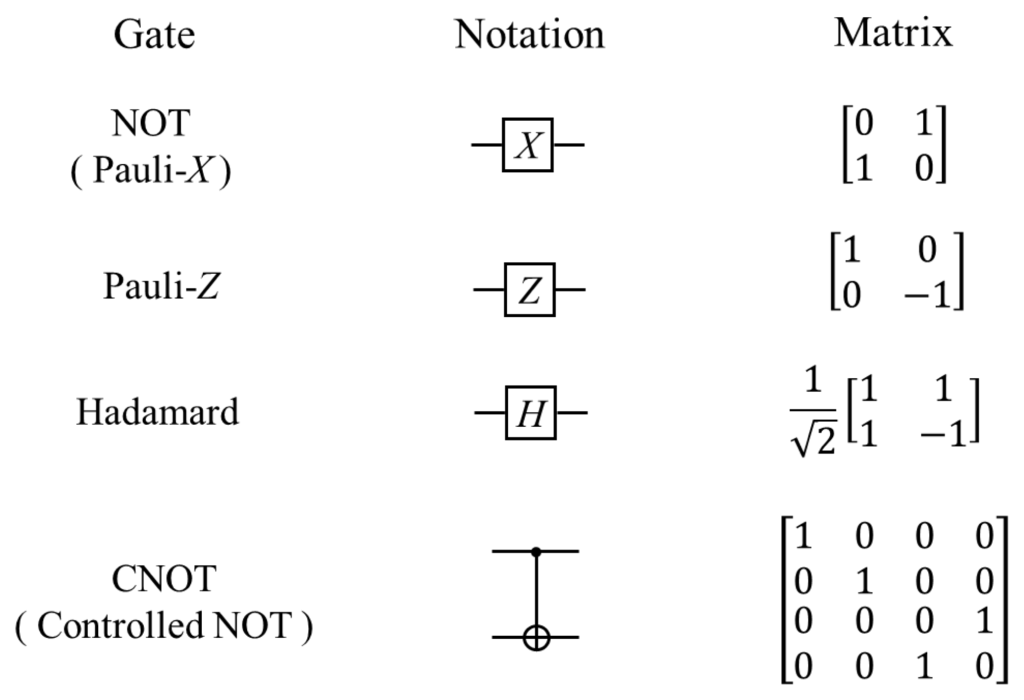
\includegraphics[scale=1.3]{gates}
			\label{fig:gates gates}
		\end{figure}

\end{frame}
%%%%%%%%%%%%%%%%%%%%%%%%%%%%%%%%%%%%%%%%%%%%%%%%%%%%%%%%%%%%%%%%%%%%%%%%%%%%%%%%%%%%%%%%%%%%%%%%%%


%%%%%%%%%%%%%%%%%%%%%%%%%%%%%%%%%%%%%%%%%%%%%%%%%%%%%%%%%%%%%%%%%%%%%%%%%%%%%%%%%%%%%%%%%%%%%%%%%%% 
\begin{frame}
	\frametitle{Unitary transformation}
		\framesubtitle{Definition}
		\vspace{-1cm}
	{\normalsize
	\hspace{0.5cm}{Unitary transformation is transformation  that preserves the inner product (isometry).}\\
	\vspace{0.5cm}
	 It is a bijective function:
	$$ U:H_1 \to H_2 $$
where $H_1$ and $H_2$ are Hilbert spaces, such that:\\
$$\langle Ux,Uy\rangle_{H_{2}}=\langle x,y\rangle _{H_{1}}$$
%for all $ x and y in H_{1} H_{1}$.
	}
\end{frame}
%%%%%%%%%%%%%%%%%%%%%%%%%%%%%%%%%%%%%%%%%%%%%%%%%%%%%%%%%%%%%%%%%%%%%%%%%%%%%%%%%%%%%%%%%%%%%%%%%%%

\subsection{Grover} 
%%%%%%%%%%%%%%%%%%%%%%%%%%%%%%%%%%%%%%%%%%%%%%%%%%%%%%%%%%%%%%%%%%%%%%%%%%%%%%%%%%%%%%%%%%%%%%%%%%%
\begin{frame}
	\frametitle{Grover's database search}
		\framesubtitle{}

		{\normalsize
		\hspace{0.5cm}{Grover's database search uses ability of quantum computing to parallel process of qubits. The algorithm allows us to find selected element in unsorted set with complexity $\sqrt{n}$.}\\
		}
		

\end{frame}
%%%%%%%%%%%%%%%%%%%%%%%%%%%%%%%%%%%%%%%%%%%%%%%%%%%%%%%%%%%%%%%%%%%%%%%%%%%%%%%%%%%%%%%%%%%%%%%%%%%

%%%%%%%%%%%%%%%%%%%%%%%%%%%%%%%%%%%%%%%%%%%%%%%%%%%%%%%%%%%%%%%%%%%%%%%%%%%%%%%%%%%%%%%%%%%%%%%%%%%
\begin{frame}
	\frametitle{Grover's database search}
		\framesubtitle{Scheme}
	\vspace{0.5cm}
		\begin{figure}
		\centering
		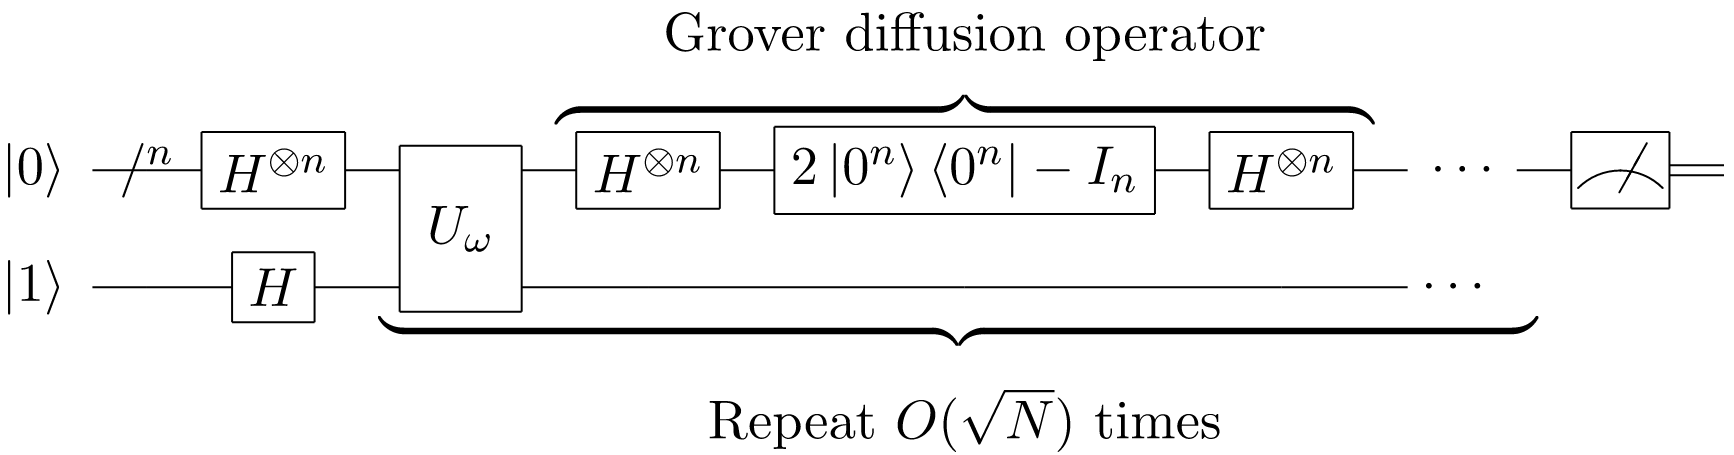
\includegraphics[width=10cm]{grdiffusion}
		\label{fig:grdiffusion grdiffusion}
	\end{figure}
\end{frame}
%%%%%%%%%%%%%%%%%%%%%%%%%%%%%%%%%%%%%%%%%%%%%%%%%%%%%%%%%%%%%%%%%%%%%%%%%%%%%%%%%%%%%%%%%%%%%%%%%%
